\subsubsection*{Analysis}
\begin{tabular}{@{}l l}
\textbf{Scope}:&The AuctionHouse\textsuperscript{TM} automated administration system\\
\textbf{Level}:&User goal\\
\textbf{Primary Actor}:&Owner\\
\textbf{Stakeholders and Interests}:&\begin{tabular}[t]{@{}l}
	Owner: wants to register the search request.\\
	Buyers: want their search request to be registered by the owner.\end{tabular}\\
\textbf{Preconditions}:&User is identified and authenticated.\\
\textbf{Postconditions}:&\begin{tabular}[t]{@{}l}
	The search request is registered in the system.\\
	The buyer is notified of confirmation or failure.\end{tabular}\\
\textbf{Special requirements}:&\begin{tabular}[t]{@{}l}A yearly fee of 20 euros must be paid for the service to process the request.\\The system should check whether this is in order.\end{tabular}\\
\textbf{Frequency of occurence}:& \begin{tabular}[t]{@{}l}Varies greatly, from 3 times a day, to once a week.\\Estimated to be 12 times per month.\footnotemark\end{tabular}
\end{tabular}\\\\
\footnotetext{The numbers came from a contact session with John. Session details are in the references, page \pageref{conv1}}
\textsl{Main Success Scenario}
\begin{enumerate}[noitemsep]
	\item The user starts the `file search request' transaction for a buyer with the system, having all parameters of the user to be added ready.
	\item The system confirms the buyer has paid the yearly fee
	\item The system confirms the interaction and asks the user to provide an item catalogue and a maximum price.
	\item The user provides these parameters.
	\item The system creates the search request with the item catalogue,the maximum price and the buyer interested and adds it to the list. The system also generates a Search ID for reference.
	\item The system informs the buyer that the request has been made.
	\item The system returns to the user with a confirmation message containing the Search ID, or a failure.
\end{enumerate}
\textsl{Extensions}
\begin{itemize}[noitemsep]
	\item If the yearly fee has not been paid, the system will return a failure and ends the transaction.
	\item When a failure is returned, the system state remains unchanged; no search request or other parameters was added.
	\item When not all required parameters were provided, the system will first ask the user to provide it until all parameters is provided.
\end{itemize}
\textsl{System Sequence Diagram}
\begin{figure}[H]
	\centering
	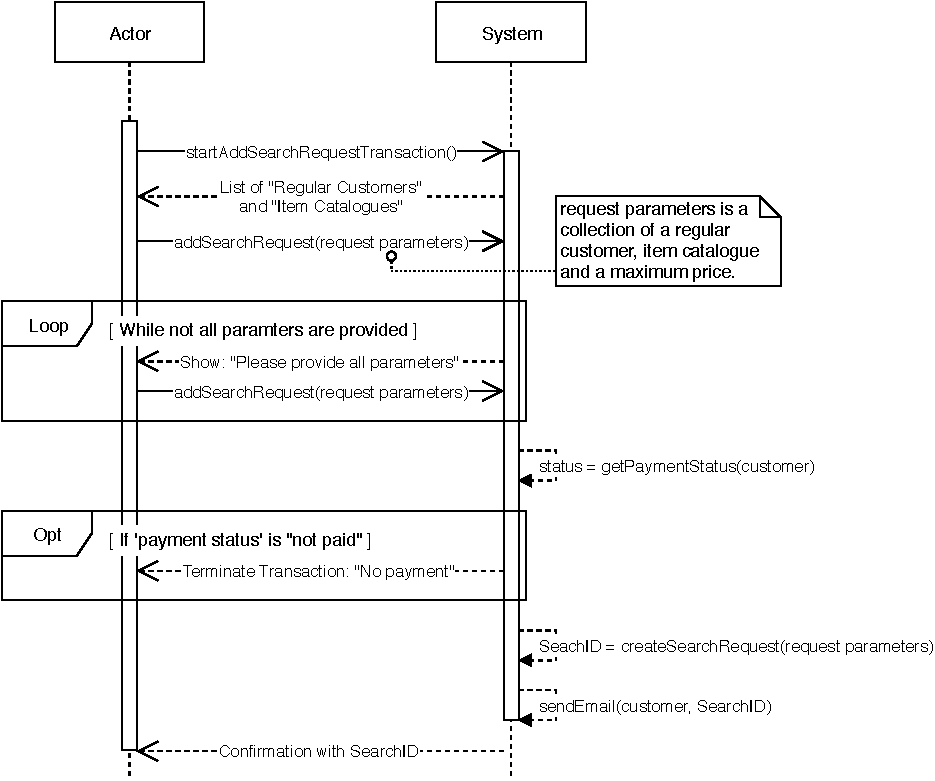
\includegraphics[scale=1]{uml/SD-bb-createsearch.pdf}
	\caption*{Interactions displayed in a System Sequence Diagram defined by the MSS and its extensions in blackbox format}
\end{figure}